
  \subsection{Programação Dinâmica}

    Programação dinâmica é uma estratégia de construção de algoritmos que 
    possui uma grande eficácia na resolução de problemas de otimização combinatória.
    Em outras palavras, essa estratégia é ideal, quando o problema original 
    é divido em subproblemas, que se repetem, logo podem ser memorizados para 
    evitar recálculo.

    Antes de aplicar essa técnica, o problema precisa atender duas propriedades:
    um problema com subproblemas(Overlapping subproblems) e uma subestrutura ideal
    (Optimal substructure).

    \begin{itemize}
      \item \textbf{Overlapping subproblems}: Uma característica também presente em divisão 
      e conquista, essa propriedade é presente em problemas, onde este pode ser 
      divido em subproblemas que são reutilizados várias vezes.
      \item \textbf{Optimal substructure}: Um problema possui uma subestrutura ideal, quando 
      uma solução ótima pode ser construída, usando solução ótima para os seus subproblemas.
    \end{itemize}

    Para melhor exemplificar esses conceitos, vamos analisar um clássico problema da computação, 
    e também um caso perfeito para ilustrar a estratégia de programação dinâmica.

    \subsubsection{Fibonnaci}

    Descobrido pelo matemático italiano do século 12, Leonardo Fibonacci, a sequência 
    fibonnaci é uma sucessão de números que aparece codificada nos mais diversos fenômenos 
    da natureza(spiral de galáxias, ciclone, conchas e vários outros). Na computação, temos 
    o problema de criar um algoritmo capaz de calcular o n° número da sequência fibonnaci.

    \begin{figure}[ht]
      \centering
      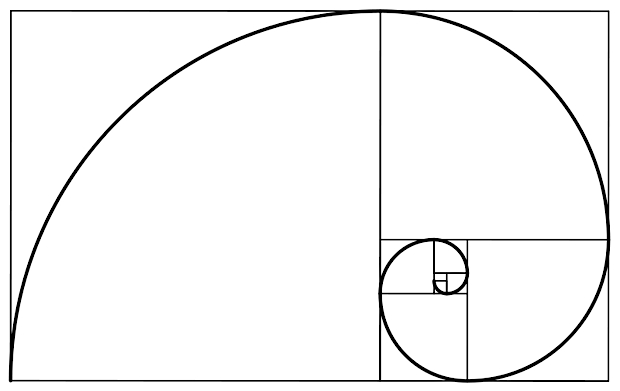
\includegraphics[width=.3\textwidth]{fibonnaci.jpg}
      \caption{Uma imagem ilustrativa da sequência Fibonnaci}
      \label{fig:fibonnaci}
    \end{figure}

    A ideia da resolução desse problema é bem simples, sabendo que a sequência inicia com 0 e 1, os
    próximos números serão sempre a soma dos dois números anteriores. A seguir temos um exemplo 
    de uma implementação ingênua do algoritmo da sequência de fibonnaci. 



    